\documentclass[../Article_Model_Parameters.tex]{subfiles}
\graphicspath{{\subfix{../Figures/}}}
\begin{document}
	
	Tables \ref{tab:Constraints_2}, \ref{tab: Estimation_results_2} and Figures \ref{fig: estimation_results_2}, \ref{fig:Regression-2}, \ref{fig:Regression_tau_simga_2} and \ref{fig: estimation_results_profiles_2} describe the solution of the parameter estimation problem solved from another initial solution.
	
	\begin{table}[!h]
		\centering
		\adjustbox{max width=\columnwidth}{%
			\begin{tabular}{ lccccccc }
				\hline 
				Parameter		&$k_m$[-] 	& $D_i$[m/s$^2$] 	& $D_e^M$[m/s$^2$]	& $C_{sat}$ [kg/m$^3$] 	& $m_{total}$[g]	& $\tau$[-] 	& $\sigma$[-] \\  \hline
				Lower bound		&0	  		& 0 	  			& 0 				&	0					& 80 		 		& 0 	   		& 0 \\ 
				Upper bound		&1 			& $+\infty$ 		& $+\infty$			&	$+\infty$			& 150 				& 1 			& $+\infty$ \\ 
				Initial guess	&0.01  		& 3 	  			& 1 				&	1					& 100 		 		& 0.65 	   		& 0.4 \\  \hline
		\end{tabular} }
		\caption{Constraints and initial guess of the parameter estimation problem}
		\label{tab:Constraints_2}
	\end{table}

	\begin{table}[!h]
		\centering
		\adjustbox{max width=\columnwidth}{%
			\csvautobooktabular{Figures/Results_estimation/estimation_2.csv} }
		\caption{Parameter estimation results rounded to fifth decimal place}
		\label{tab: Estimation_results_2}
	\end{table}

	\begin{figure}[!h]
		\centering
		\begin{subfigure}[b]{\columnwidth}
			\centering
			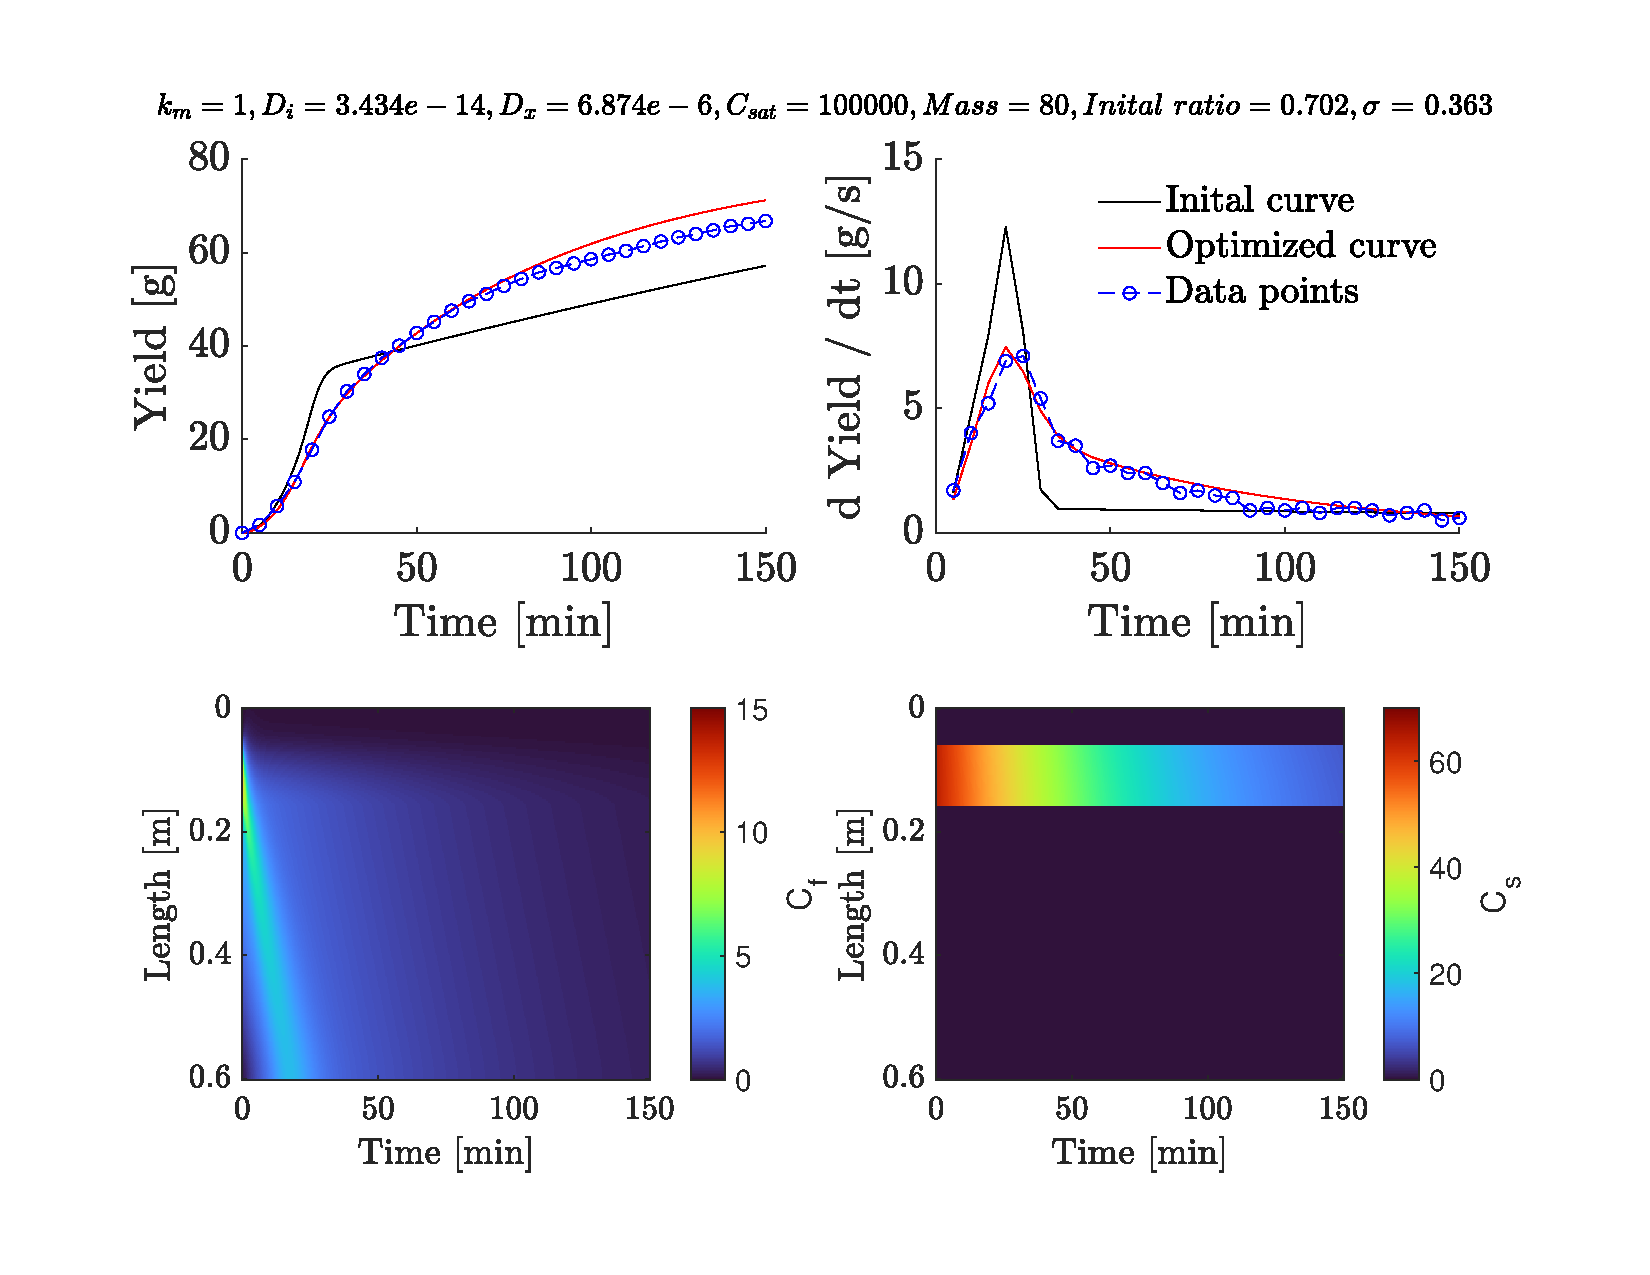
\includegraphics[trim = 2cm 10.5cm 2.5cm 2.02cm,clip,width=\textwidth]{/Results_estimation/Fitting_LUKE_T40_P200_2.pdf}
			\caption{Experiment at $40^\circ C$ and $200$ bar}
		\end{subfigure}
		\begin{subfigure}[b]{\columnwidth}
			\centering
			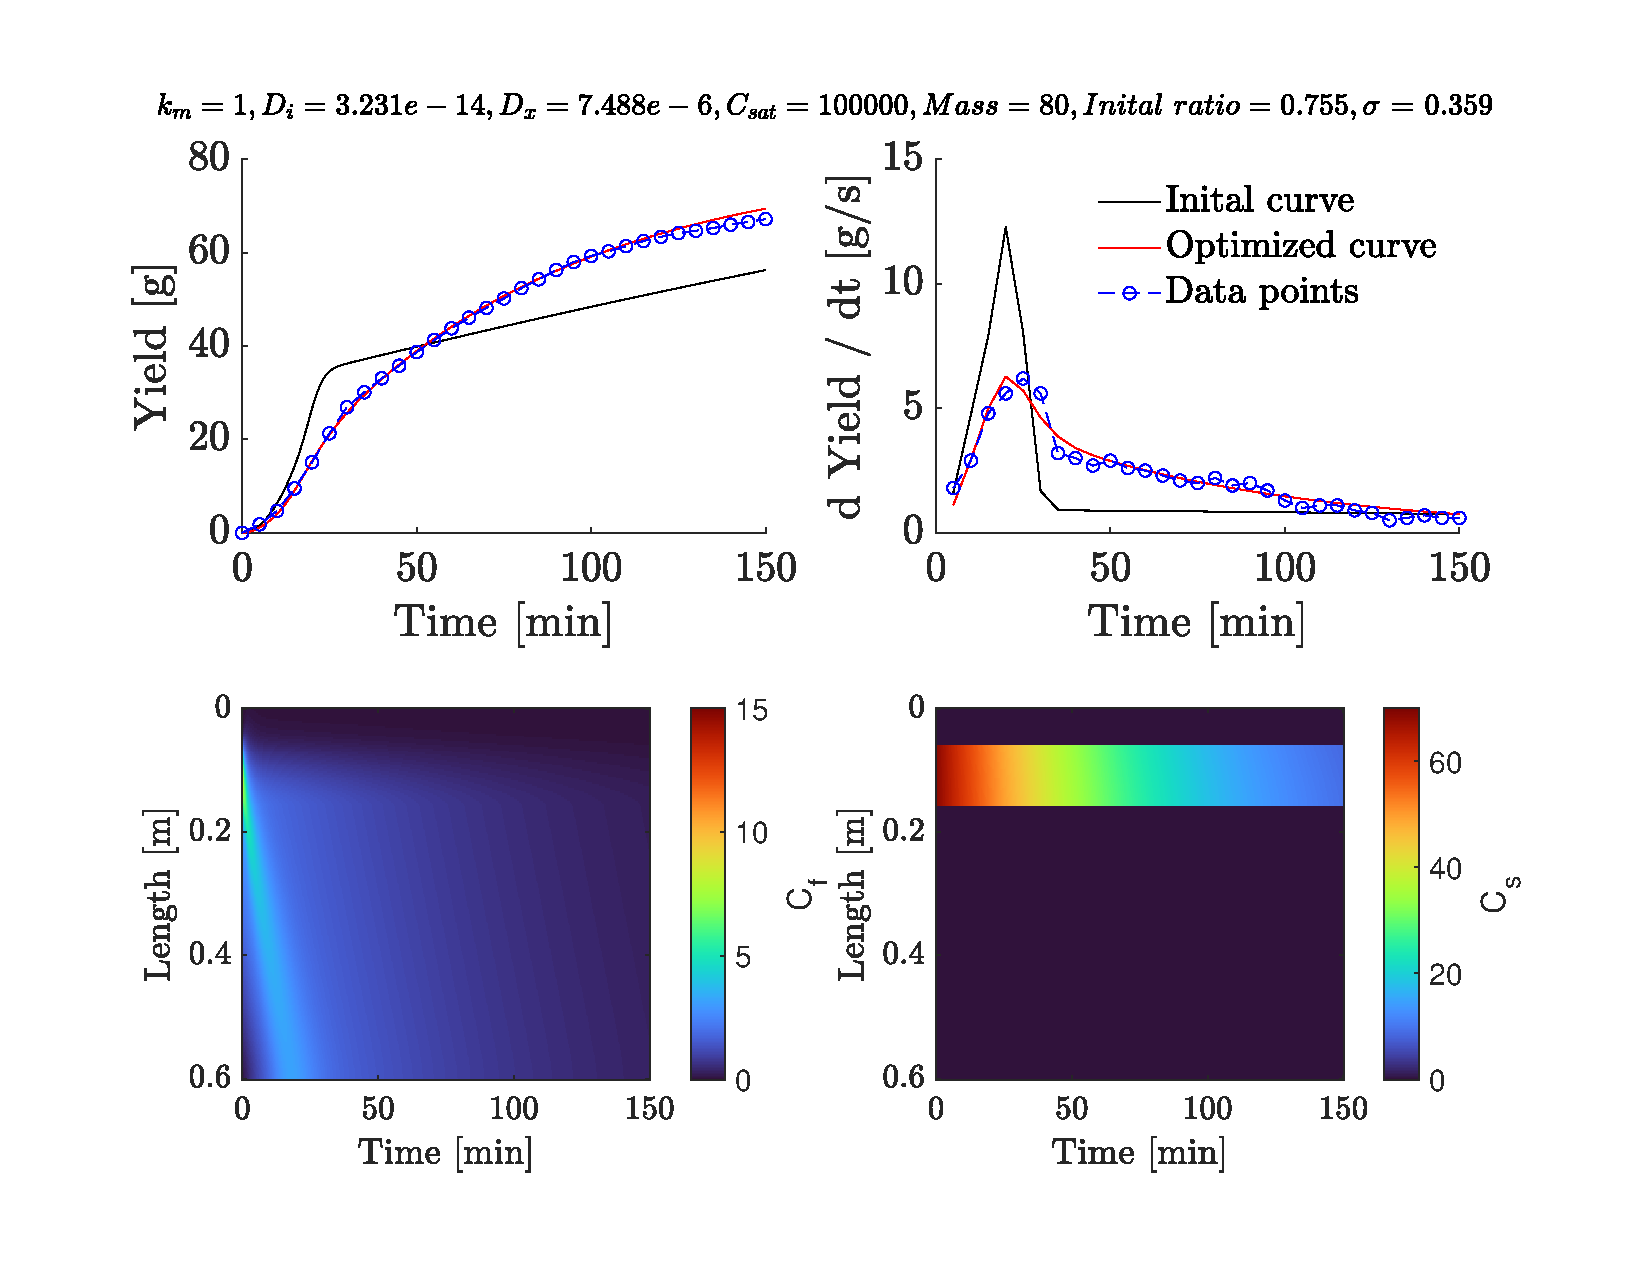
\includegraphics[trim = 2cm 10.5cm 2.5cm 2.02cm,clip,width=\textwidth]{/Results_estimation/Fitting_LUKE_T50_P200_2.pdf}
			\caption{Experiment at $50^\circ C$ and $200$ bar}
		\end{subfigure}
		\begin{subfigure}[b]{\columnwidth}
			\centering
			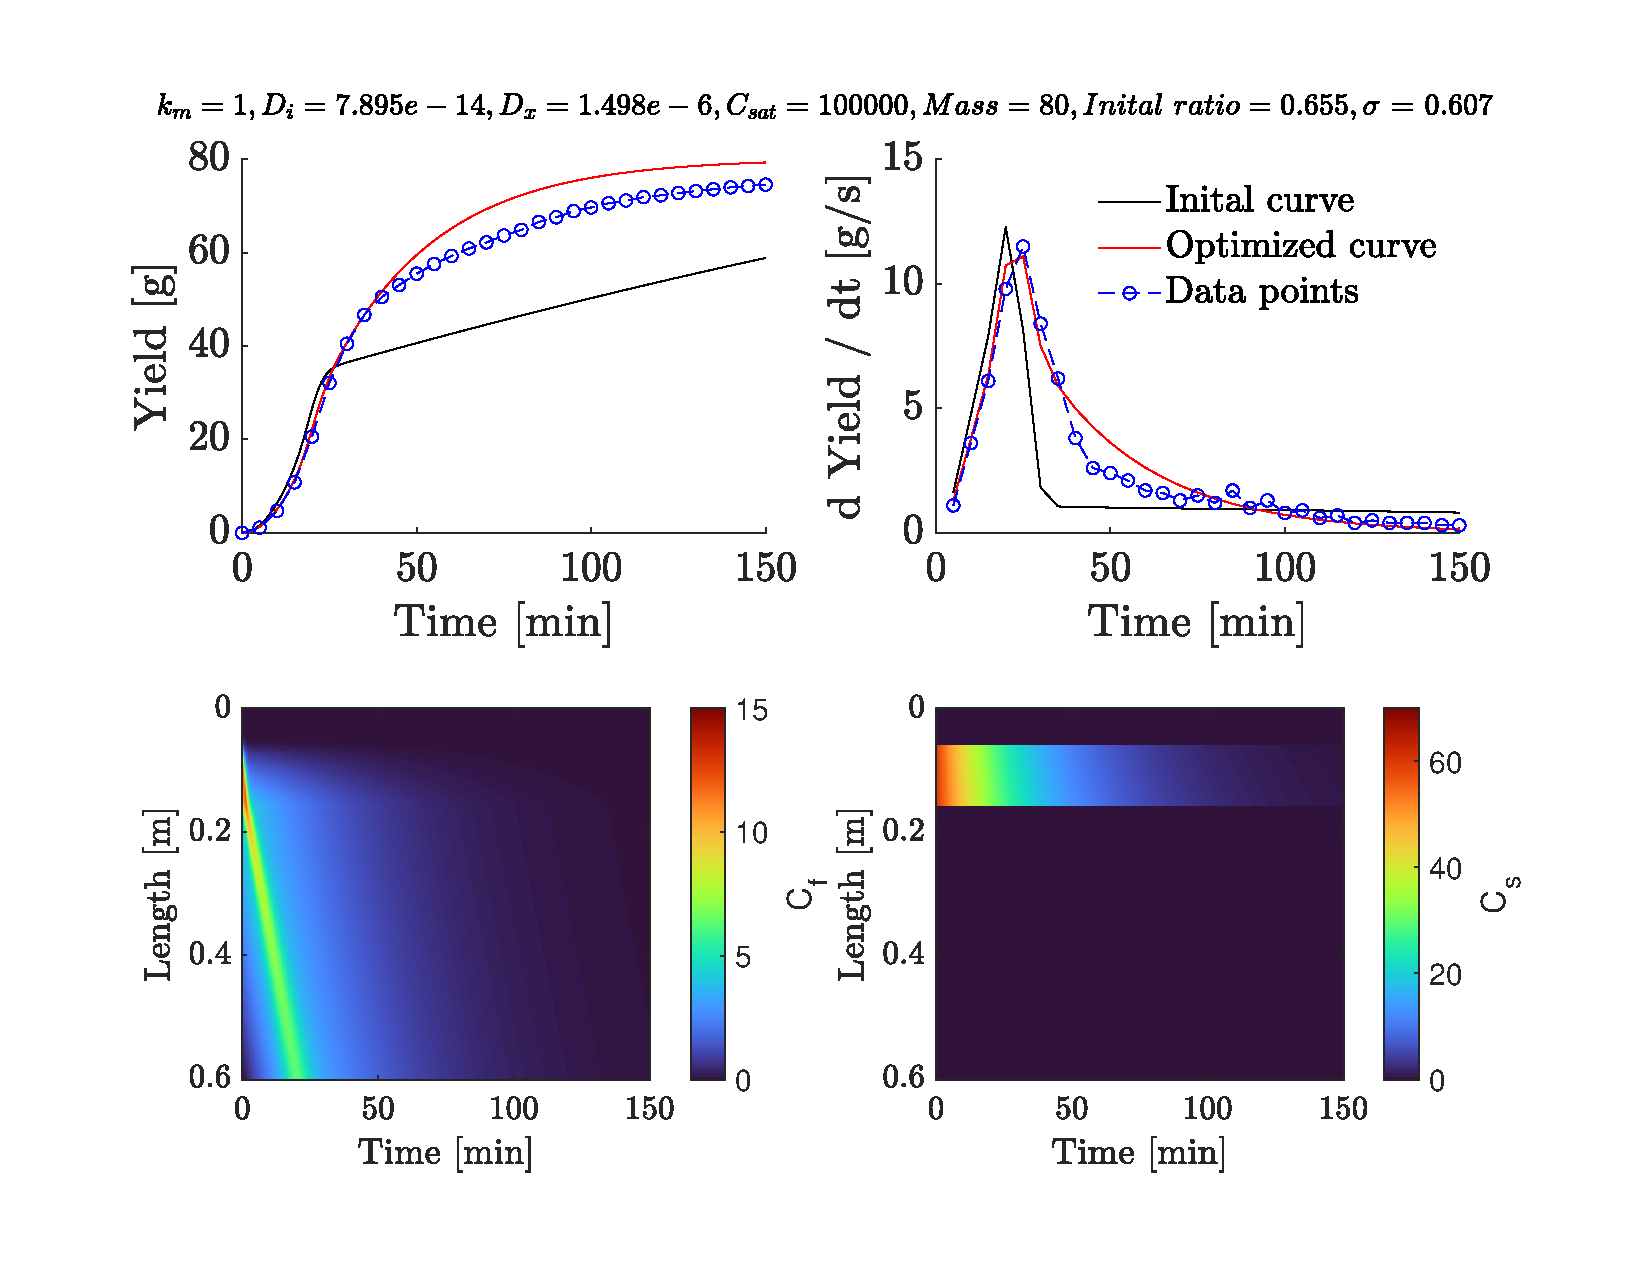
\includegraphics[trim = 2cm 10.5cm 2.5cm 2.02cm,clip,width=\textwidth]{/Results_estimation/Fitting_LUKE_T40_P300_org_2.pdf}
			\caption{Experiment at $40^\circ C$ and $300$ bar}
		\end{subfigure}
		\begin{subfigure}[b]{\columnwidth}
			\centering
			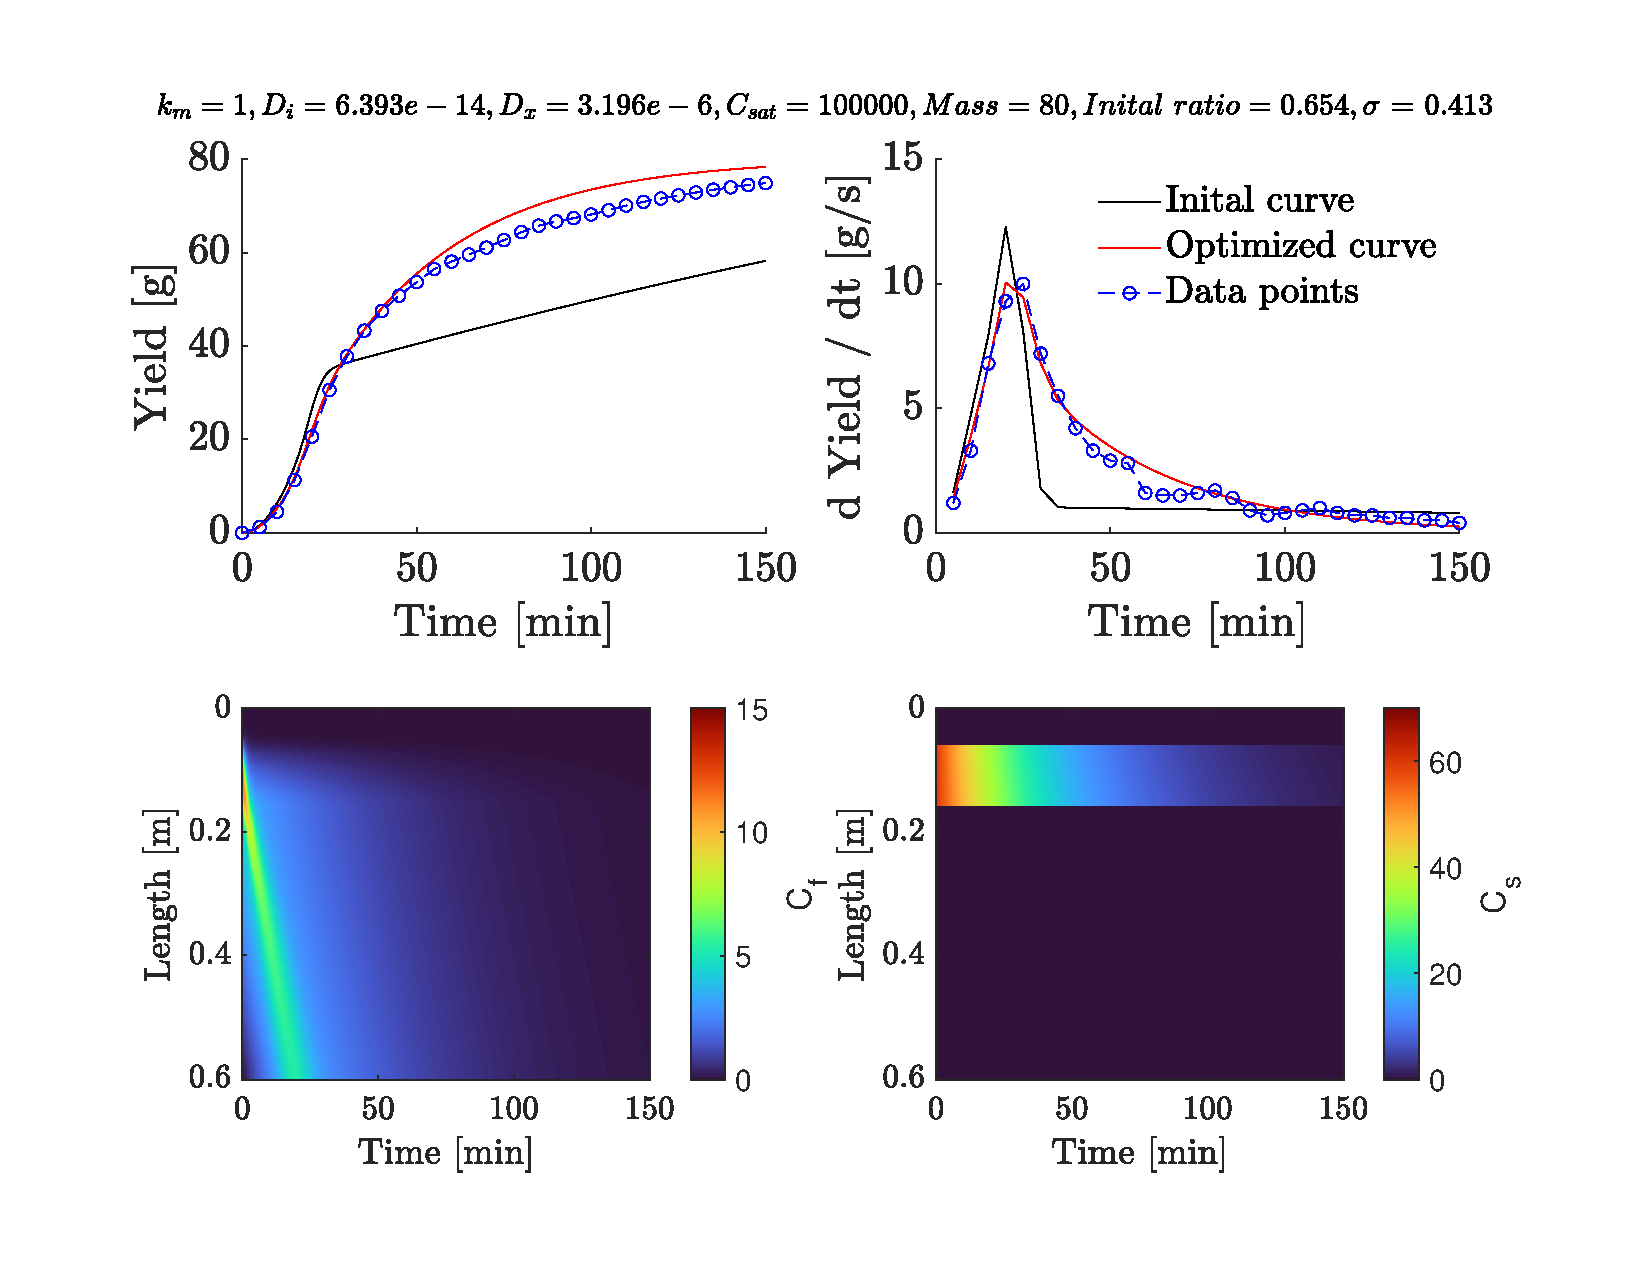
\includegraphics[trim = 2cm 10.5cm 2.5cm 2.02cm,clip,width=\textwidth]{/Results_estimation/Fitting_LUKE_T50_P300_org_2.pdf}
			\caption{Experiment at $50^\circ C$ and $300$ bar}
		\end{subfigure}
		\caption{Results of parameter fitting, with estimation of the initial state}
		\label{fig: estimation_results_2}
	\end{figure}

	\begin{figure}[!h]
		\centering
		\begin{subfigure}[b]{\columnwidth}
			\centering
			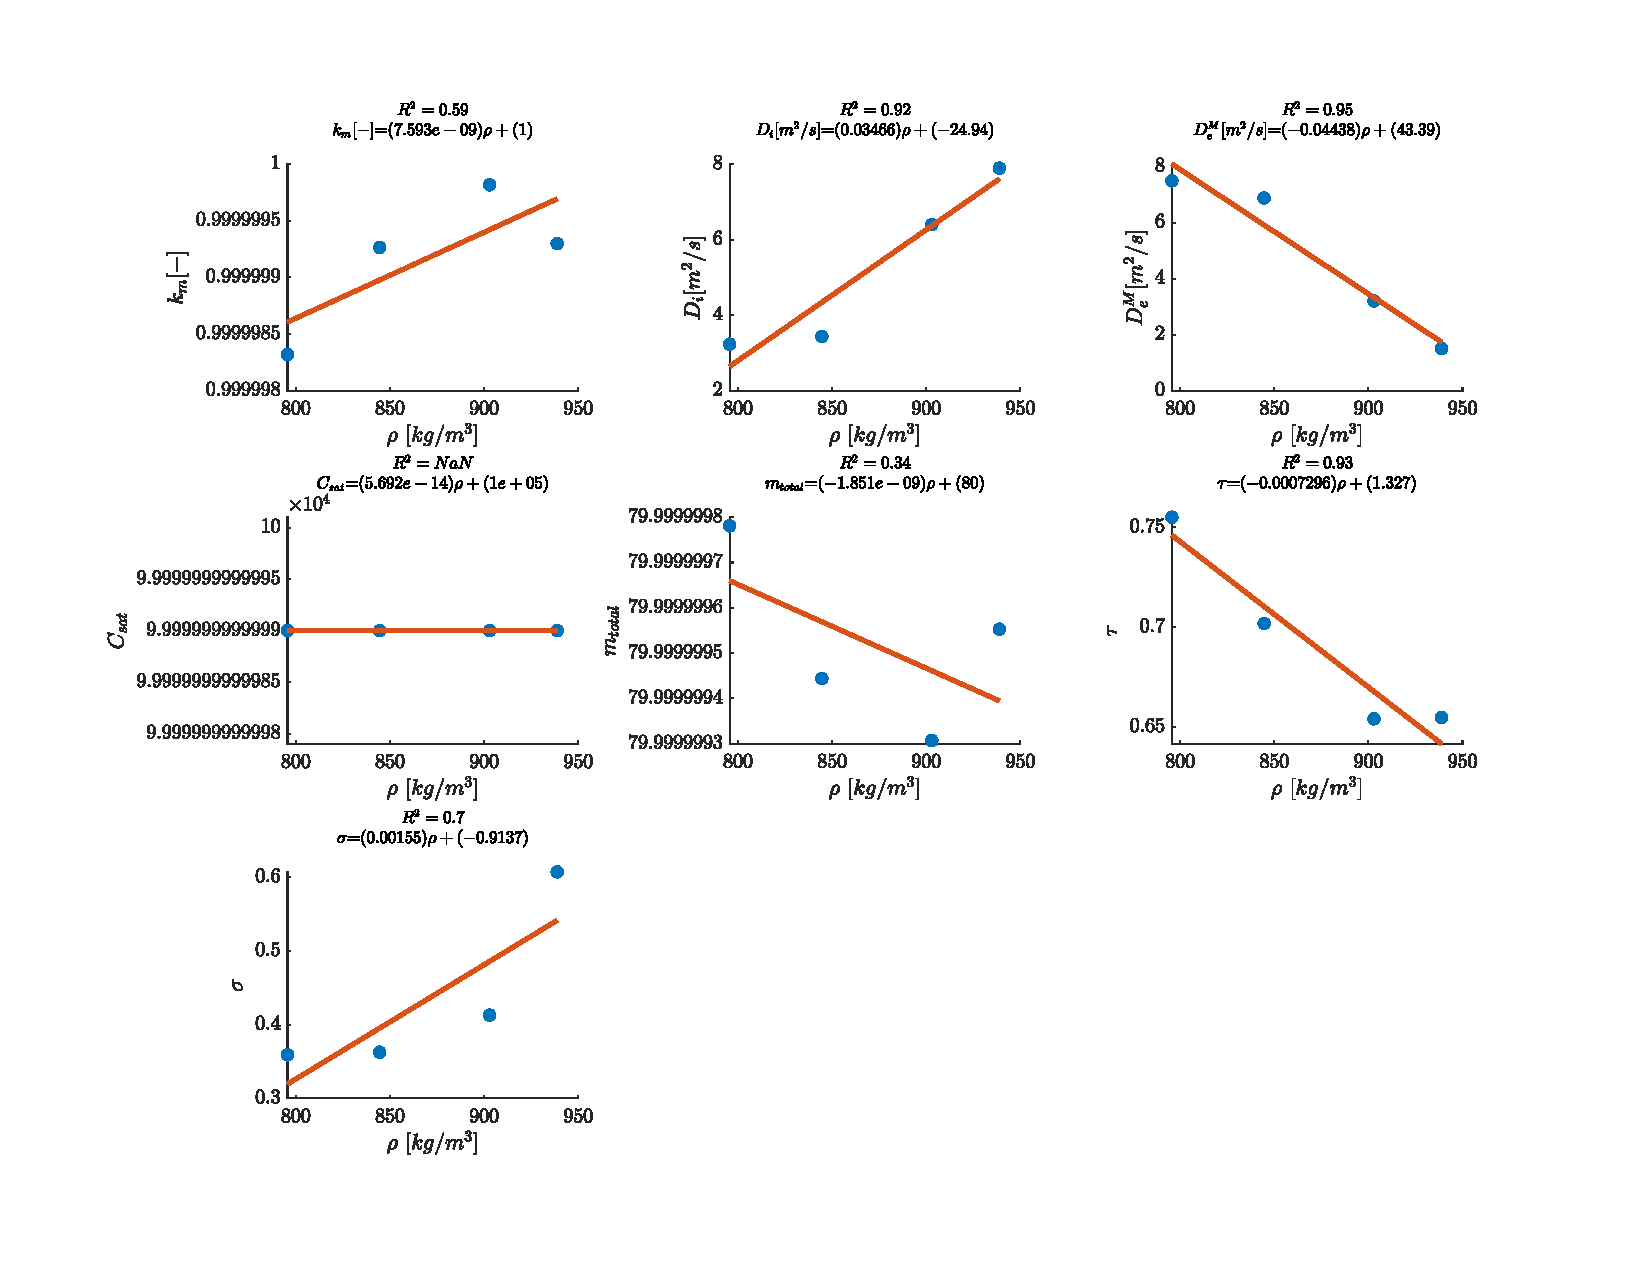
\includegraphics[trim = 11.7cm 14cm 2.3cm 1cm,clip,width=\textwidth]{/Results_estimation/Trend_Lines_order_1_2.pdf}
			\caption{First-order polynomial regression of fitted parameters ($D_i$ and $D_e^M$) as a function of fluid density $\rho_f$}
			\label{fig:Regression_12}
		\end{subfigure}
		\begin{subfigure}[b]{\columnwidth}
			\centering
			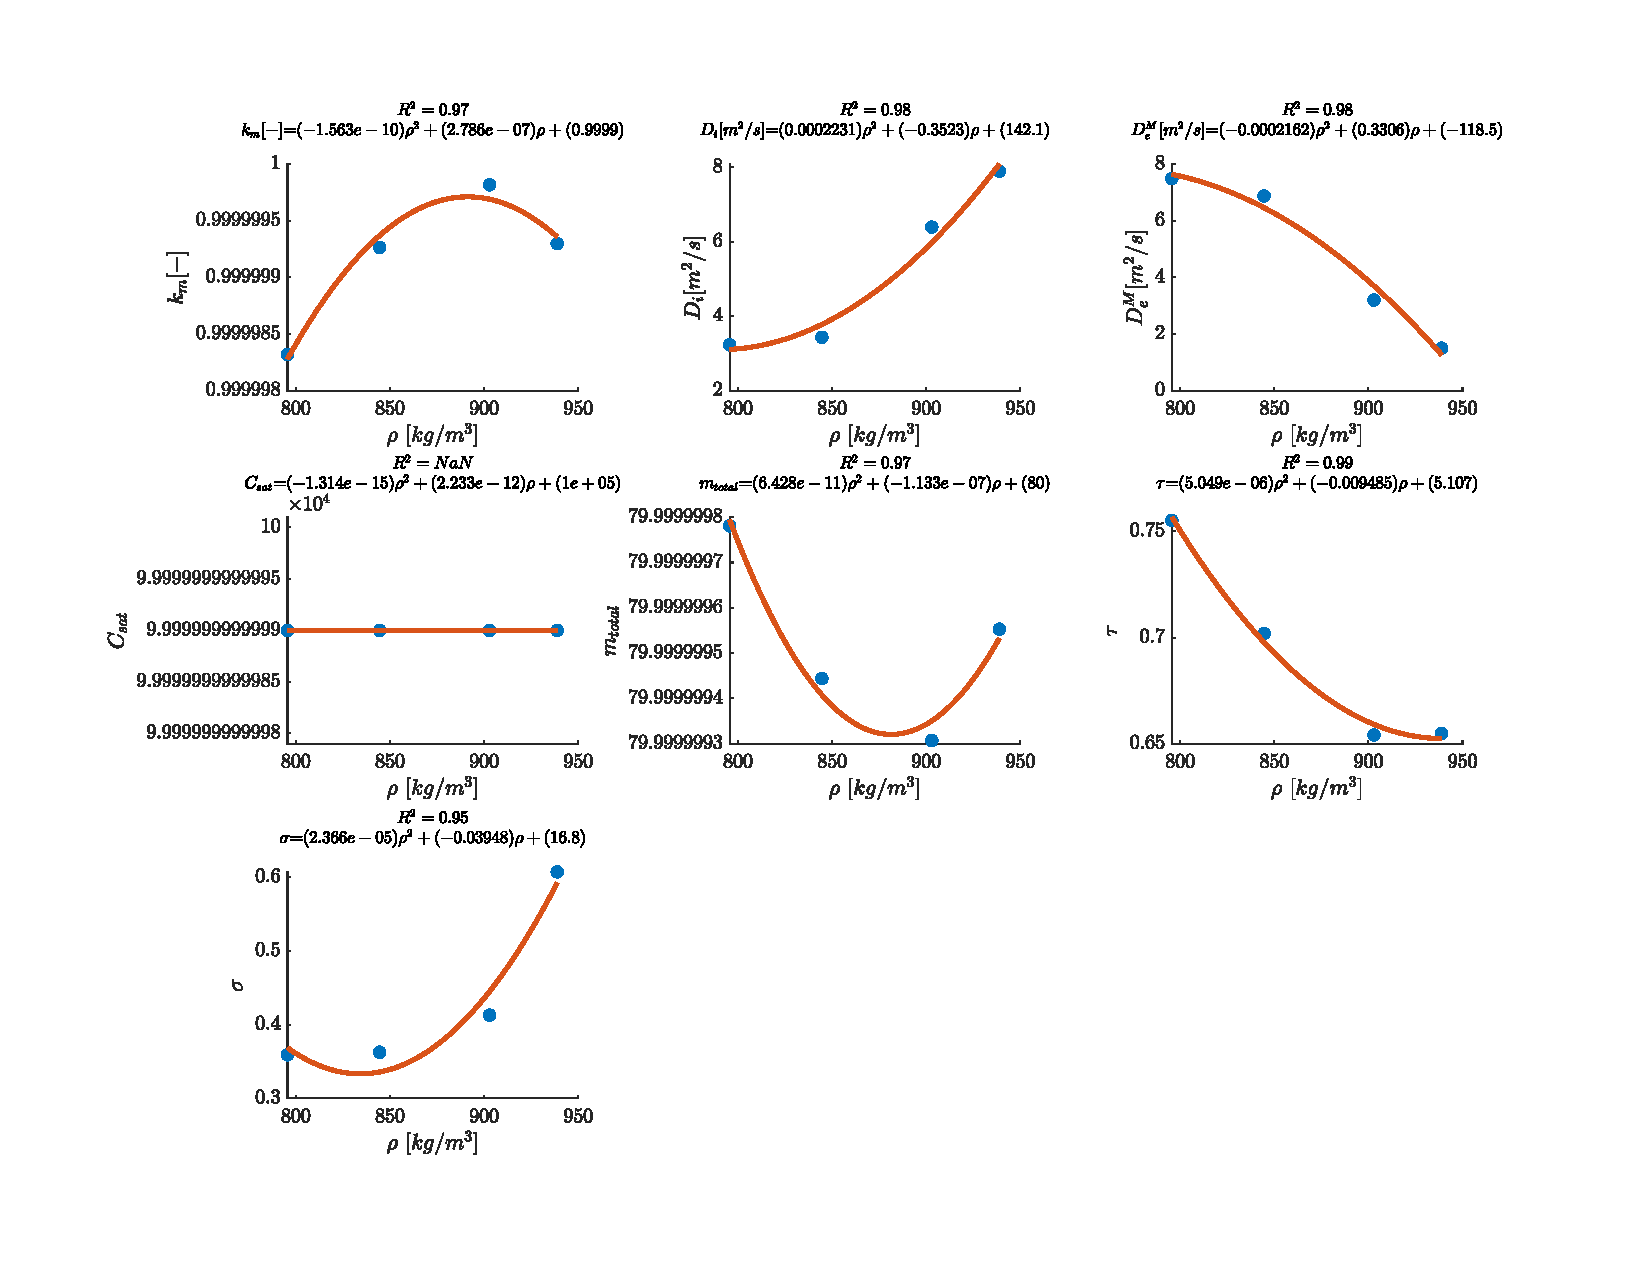
\includegraphics[trim = 11.7cm 14cm 2.3cm 1cm,clip,width=\textwidth]{/Results_estimation/Trend_Lines_order_2_2.pdf}
			\caption{Second-order polynomial regression of fitted parameters ($D_i$ and $D_e^M$) as a function of fluid density $\rho_f$}
			\label{fig:Regression_22}
		\end{subfigure}
		\caption{Regression of $D_i$ and $D_e^M$} 
		\label{fig:Regression-2}
	\end{figure}

	\begin{figure}[!h]
		\centering
		\begin{subfigure}[b]{\columnwidth}
			\centering
			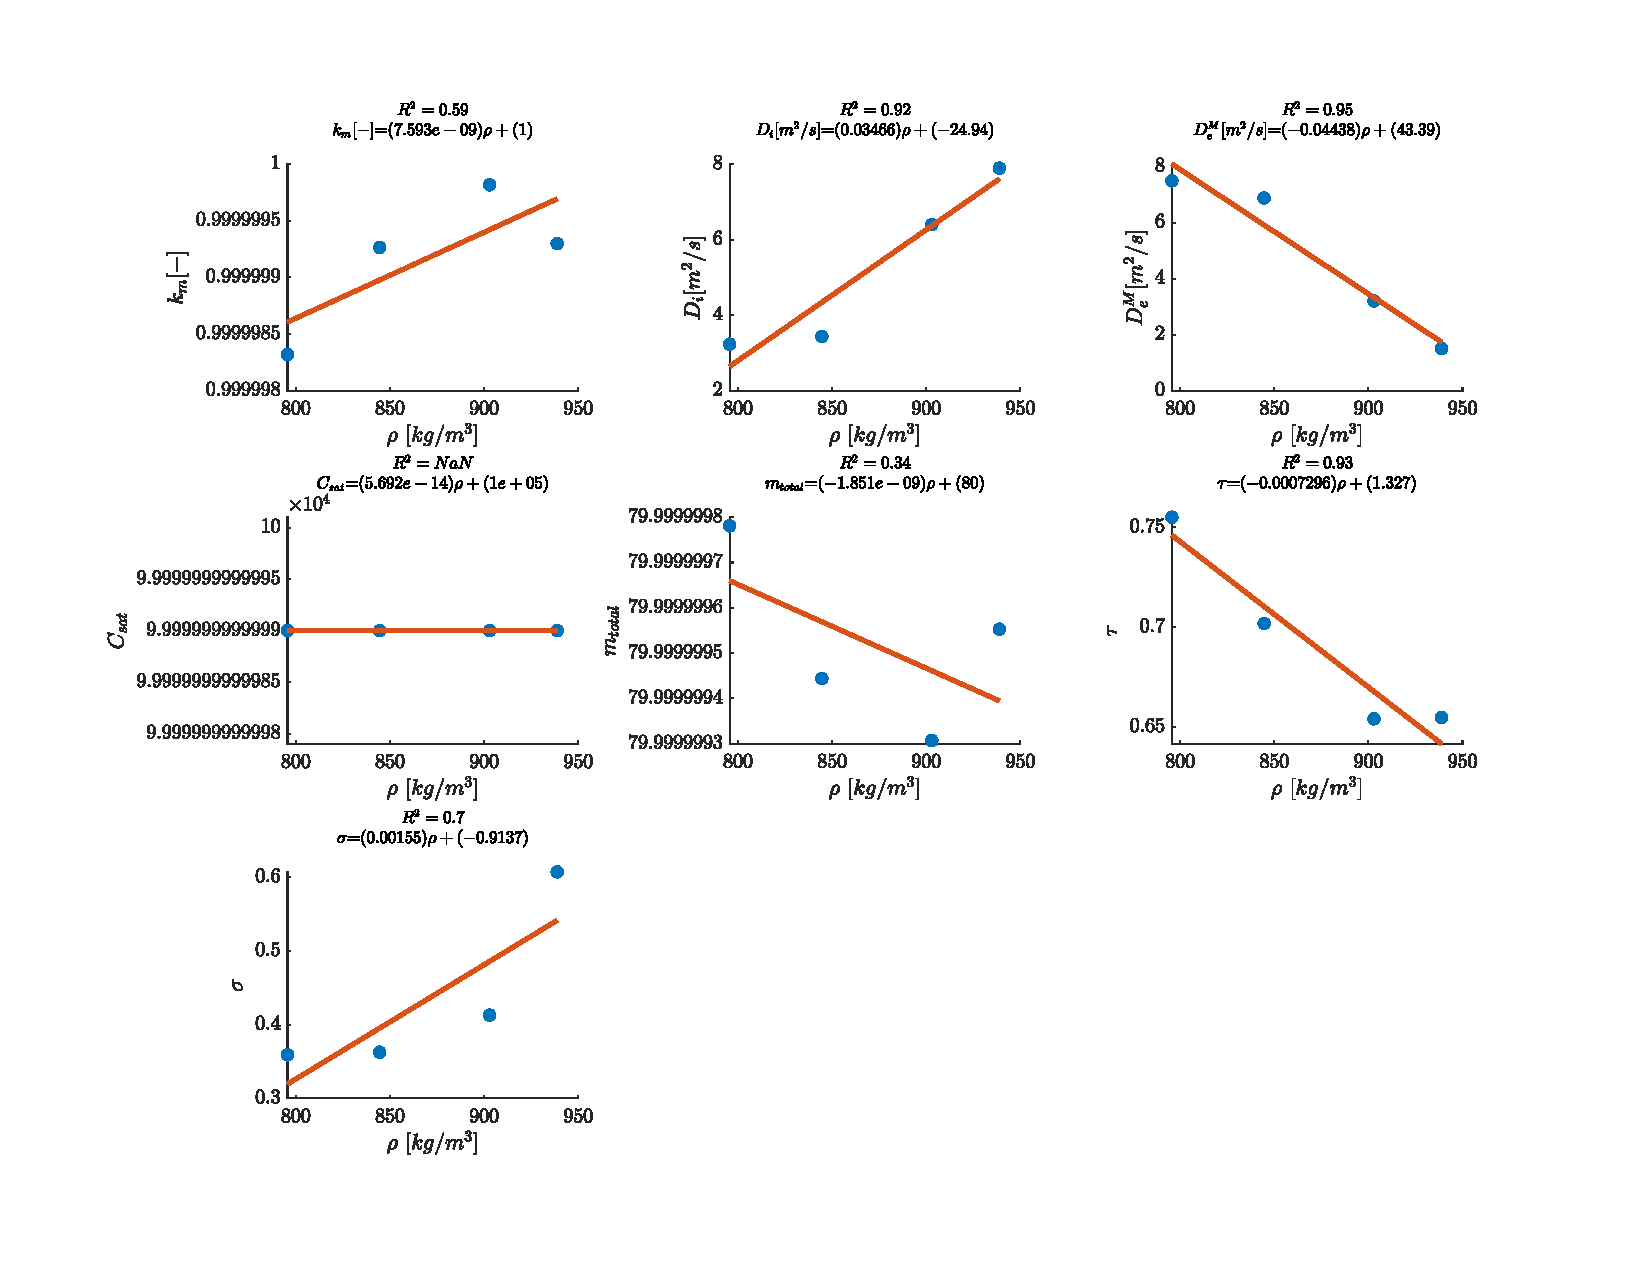
\includegraphics[trim = 18.8cm 8cm 2.5cm 7.6cm,clip,width=0.49\textwidth]{/Results_estimation/Trend_Lines_order_1_2.pdf}
			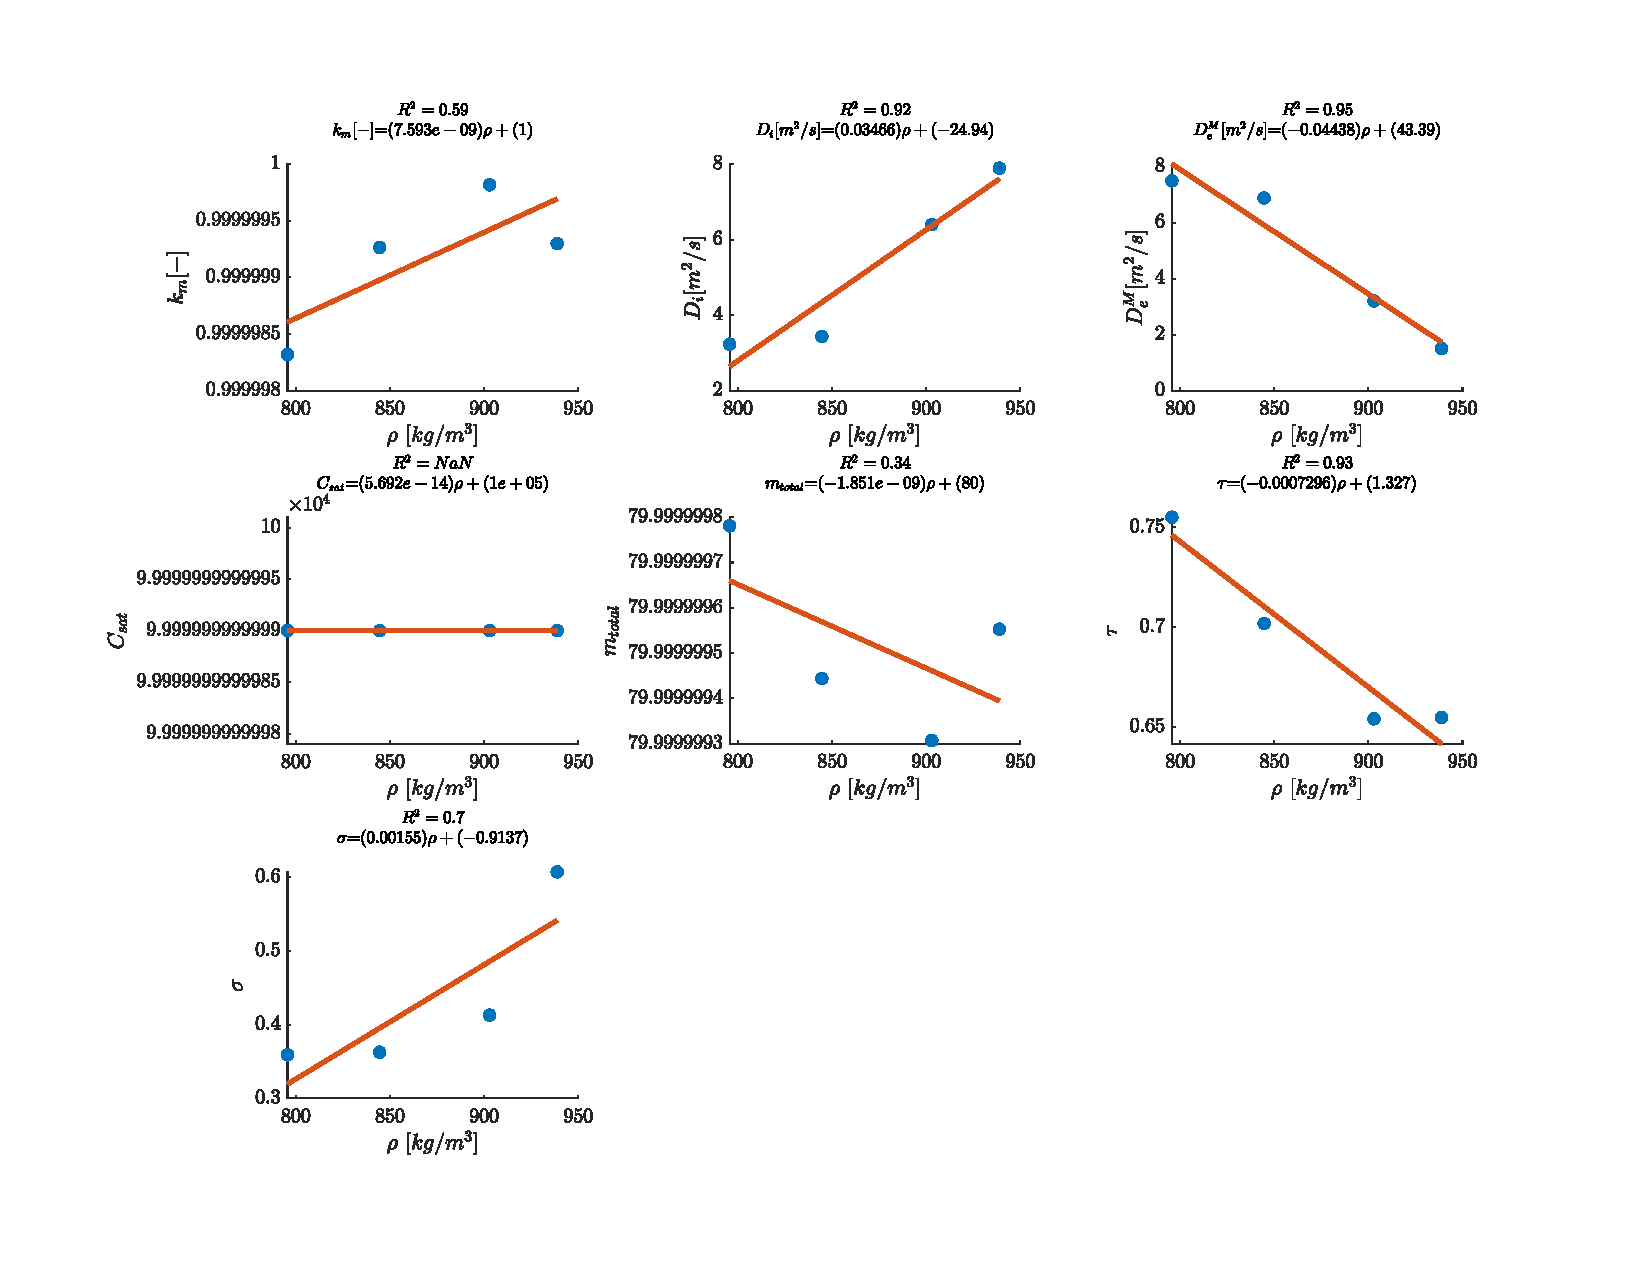
\includegraphics[trim = 4cm 2cm 17.5cm 13.6cm,clip,width=0.49\textwidth]{/Results_estimation/Trend_Lines_order_1_2.pdf}
			\caption{First order polynomial regression of fitted parameters ($\tau$ and $\sigma$) as a function of fluid density $\rho_f$}
			\label{fig:Regression_32}
		\end{subfigure}
		\begin{subfigure}[b]{\columnwidth}
			\centering
			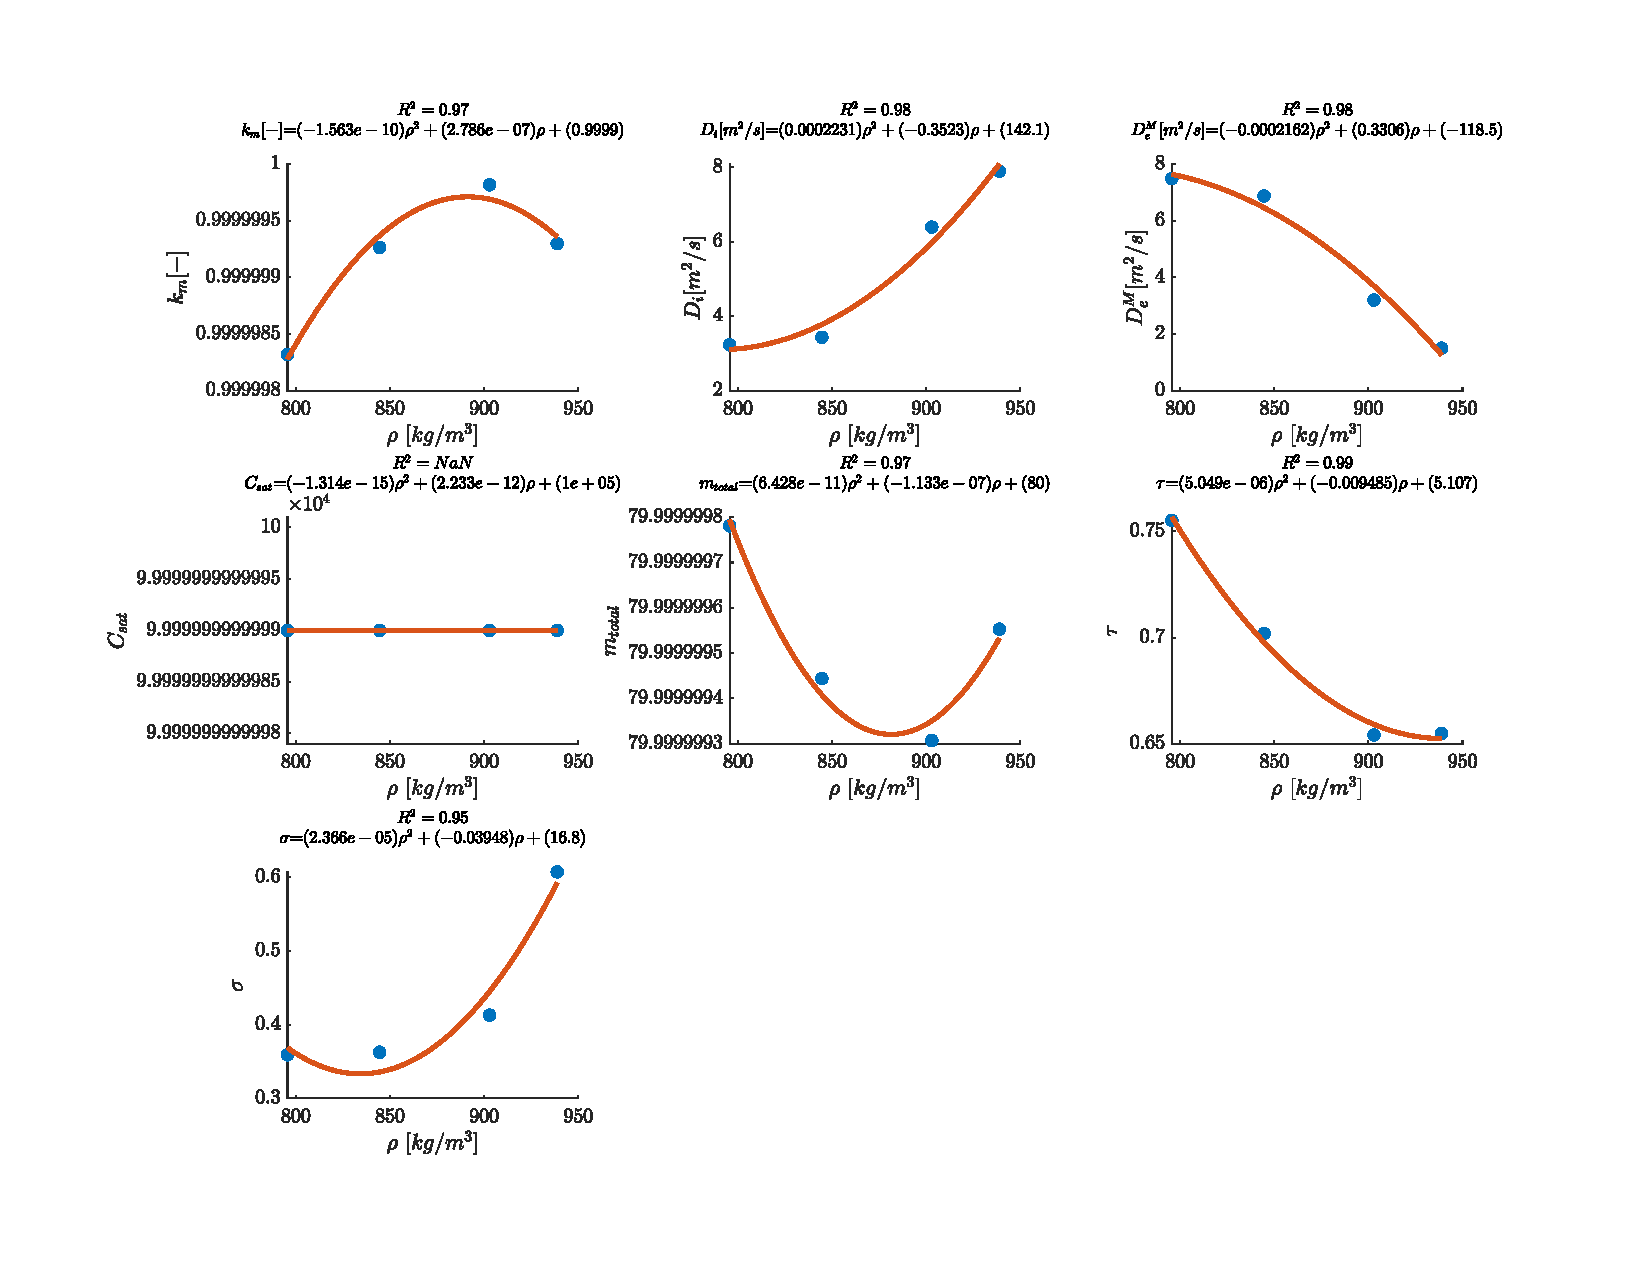
\includegraphics[trim = 18.8cm 8cm 2.5cm 7.6cm,clip,width=0.49\textwidth]{/Results_estimation/Trend_Lines_order_2_2.pdf}
			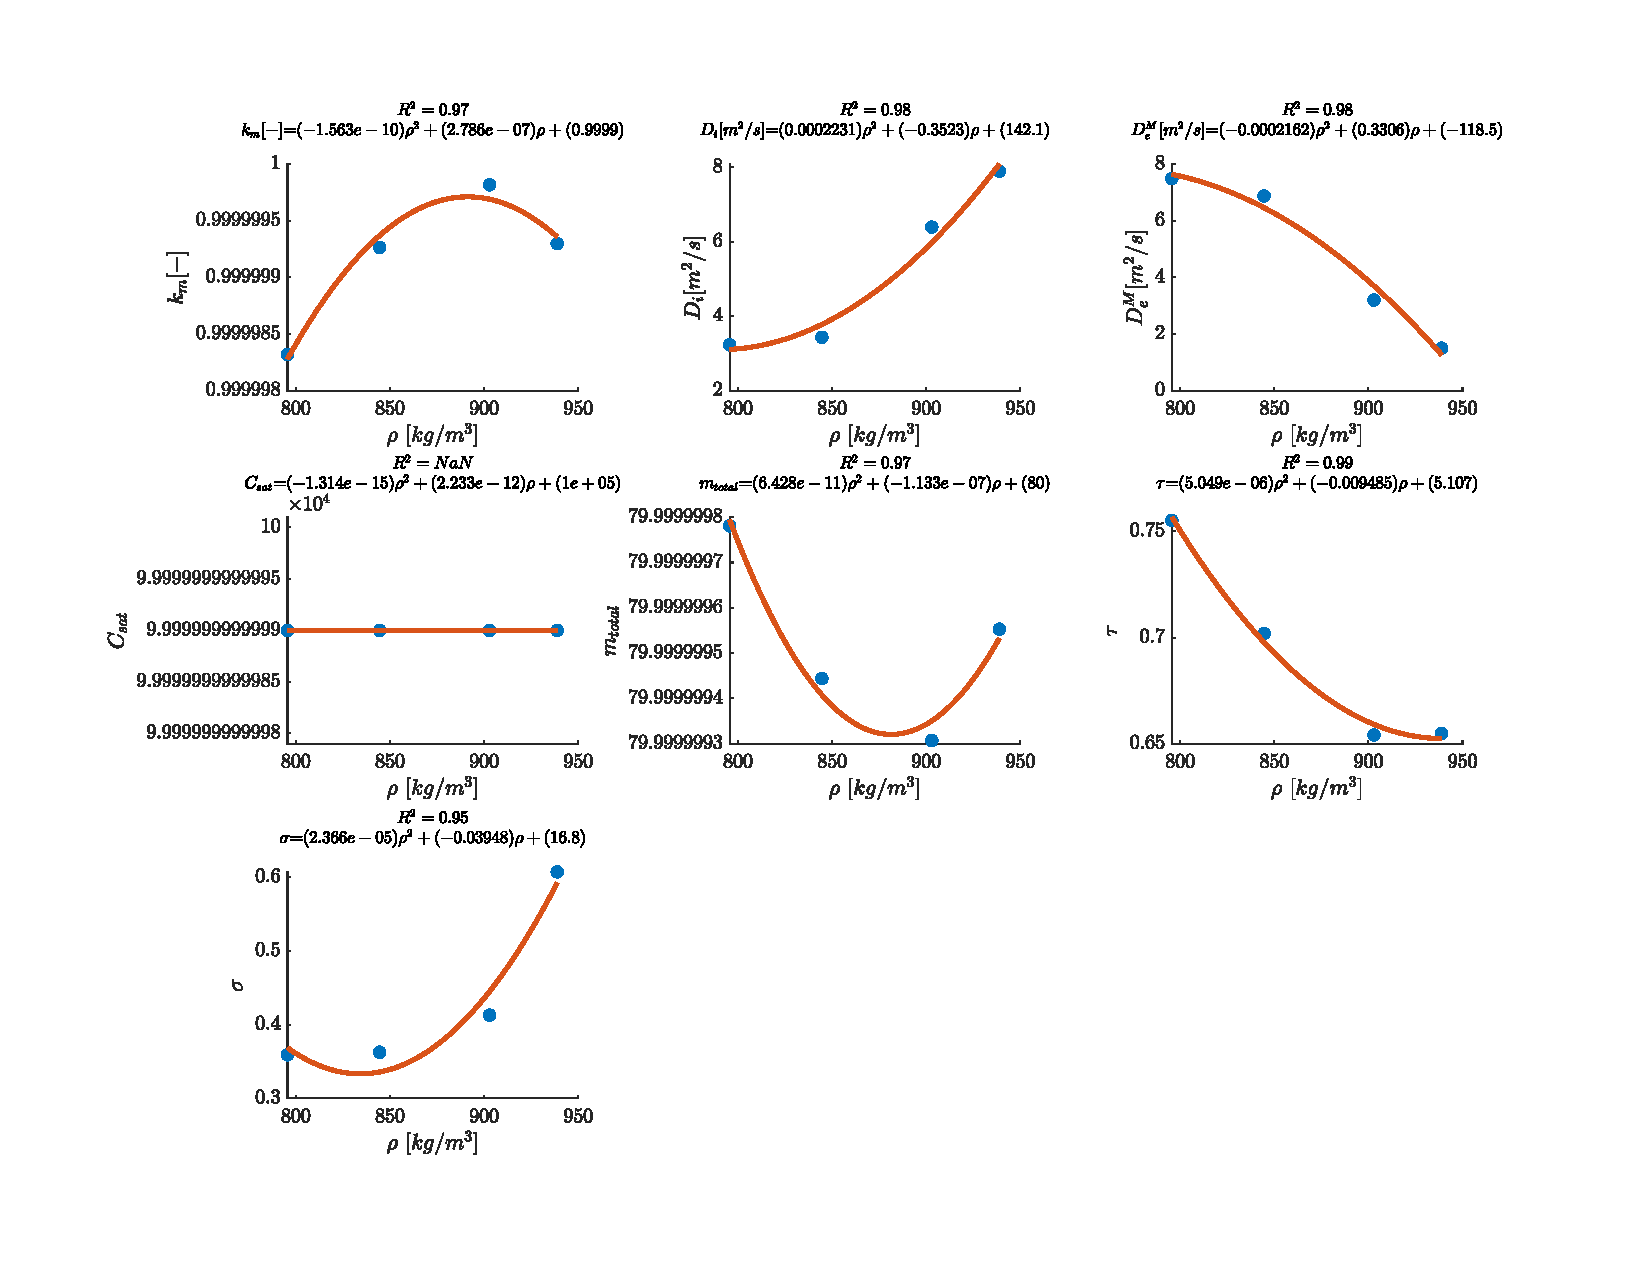
\includegraphics[trim = 4cm 2cm 17.5cm 13.6cm,clip,width=0.49\textwidth]{/Results_estimation/Trend_Lines_order_2_2.pdf}
			\caption{Second order polynomial regression of fitted parameters ($\tau$ and $\sigma$) as a function of fluid density $\rho_f$}
			\label{fig:Regression_42}
		\end{subfigure}
		\caption{Regression of $\tau$ and $\sigma$} 
		\label{fig:Regression_tau_simga_2}
	\end{figure}

	\begin{figure}[!h]
		\centering
		\begin{subfigure}[b]{\columnwidth}
			\centering
			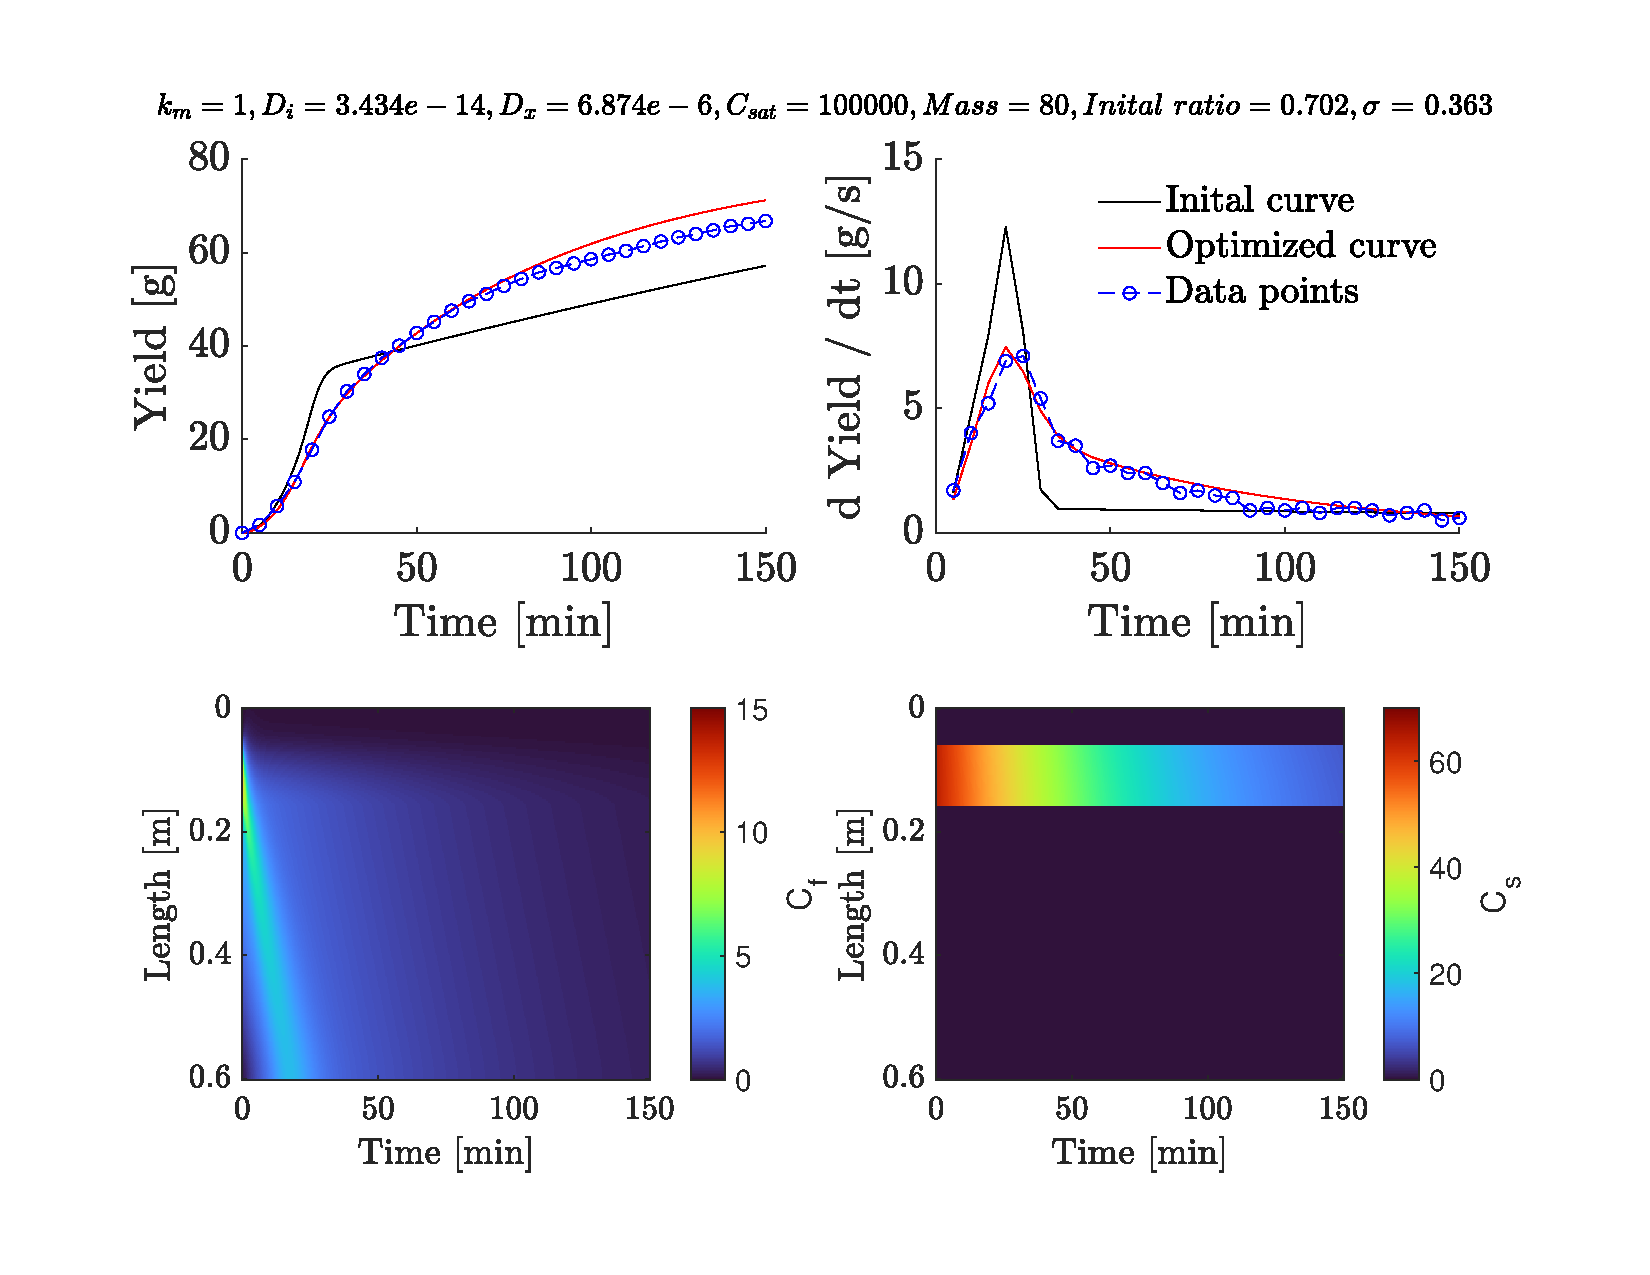
\includegraphics[trim = 2cm 1.4cm 1.9cm 11cm,clip,width=\textwidth]{/Results_estimation/Fitting_LUKE_T40_P200_2.pdf}
			\caption{Experiment at $40^\circ C$ and $200$ bar}
		\end{subfigure}
		\begin{subfigure}[b]{\columnwidth}
			\centering
			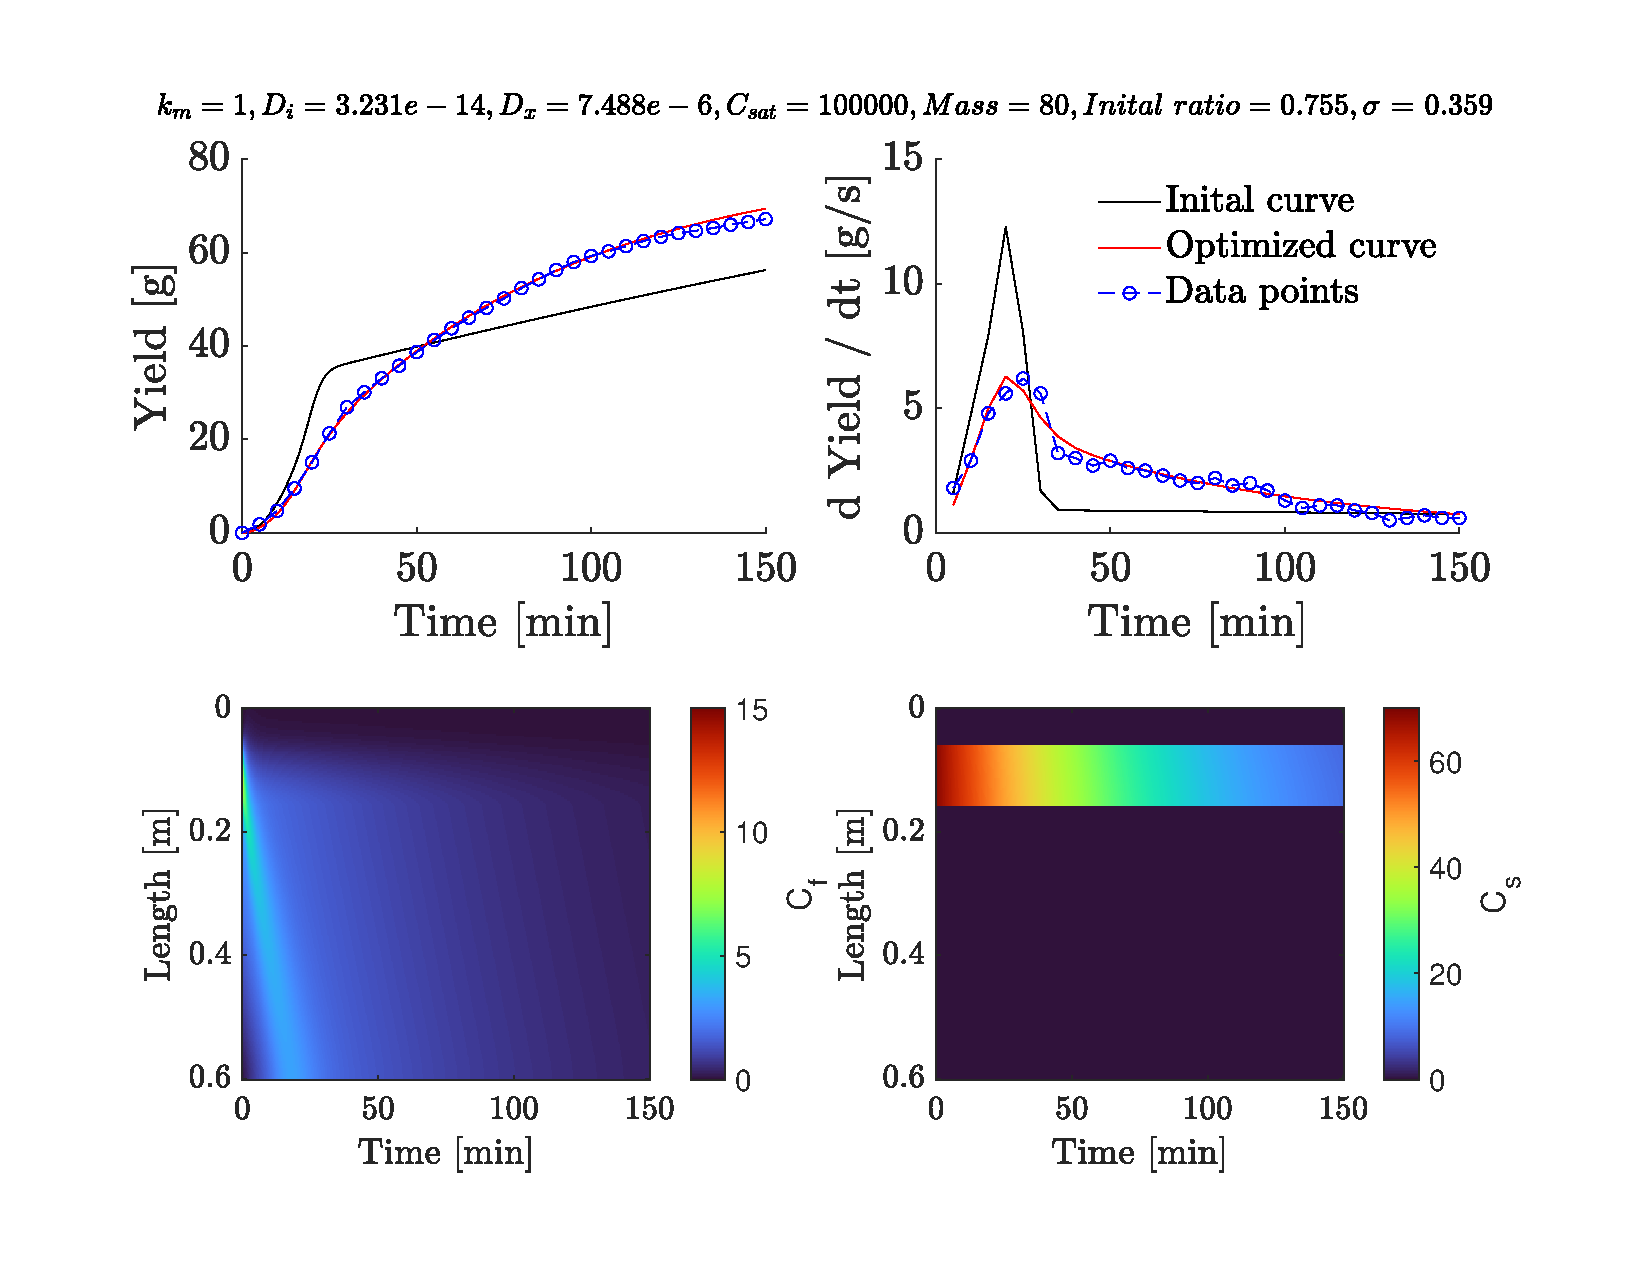
\includegraphics[trim = 2cm 1.4cm 1.9cm 11cm,clip,width=\textwidth]{/Results_estimation/Fitting_LUKE_T50_P200_2.pdf}
			\caption{Experiment at $50^\circ C$ and $200$ bar}
		\end{subfigure}
		\begin{subfigure}[b]{\columnwidth}
			\centering
			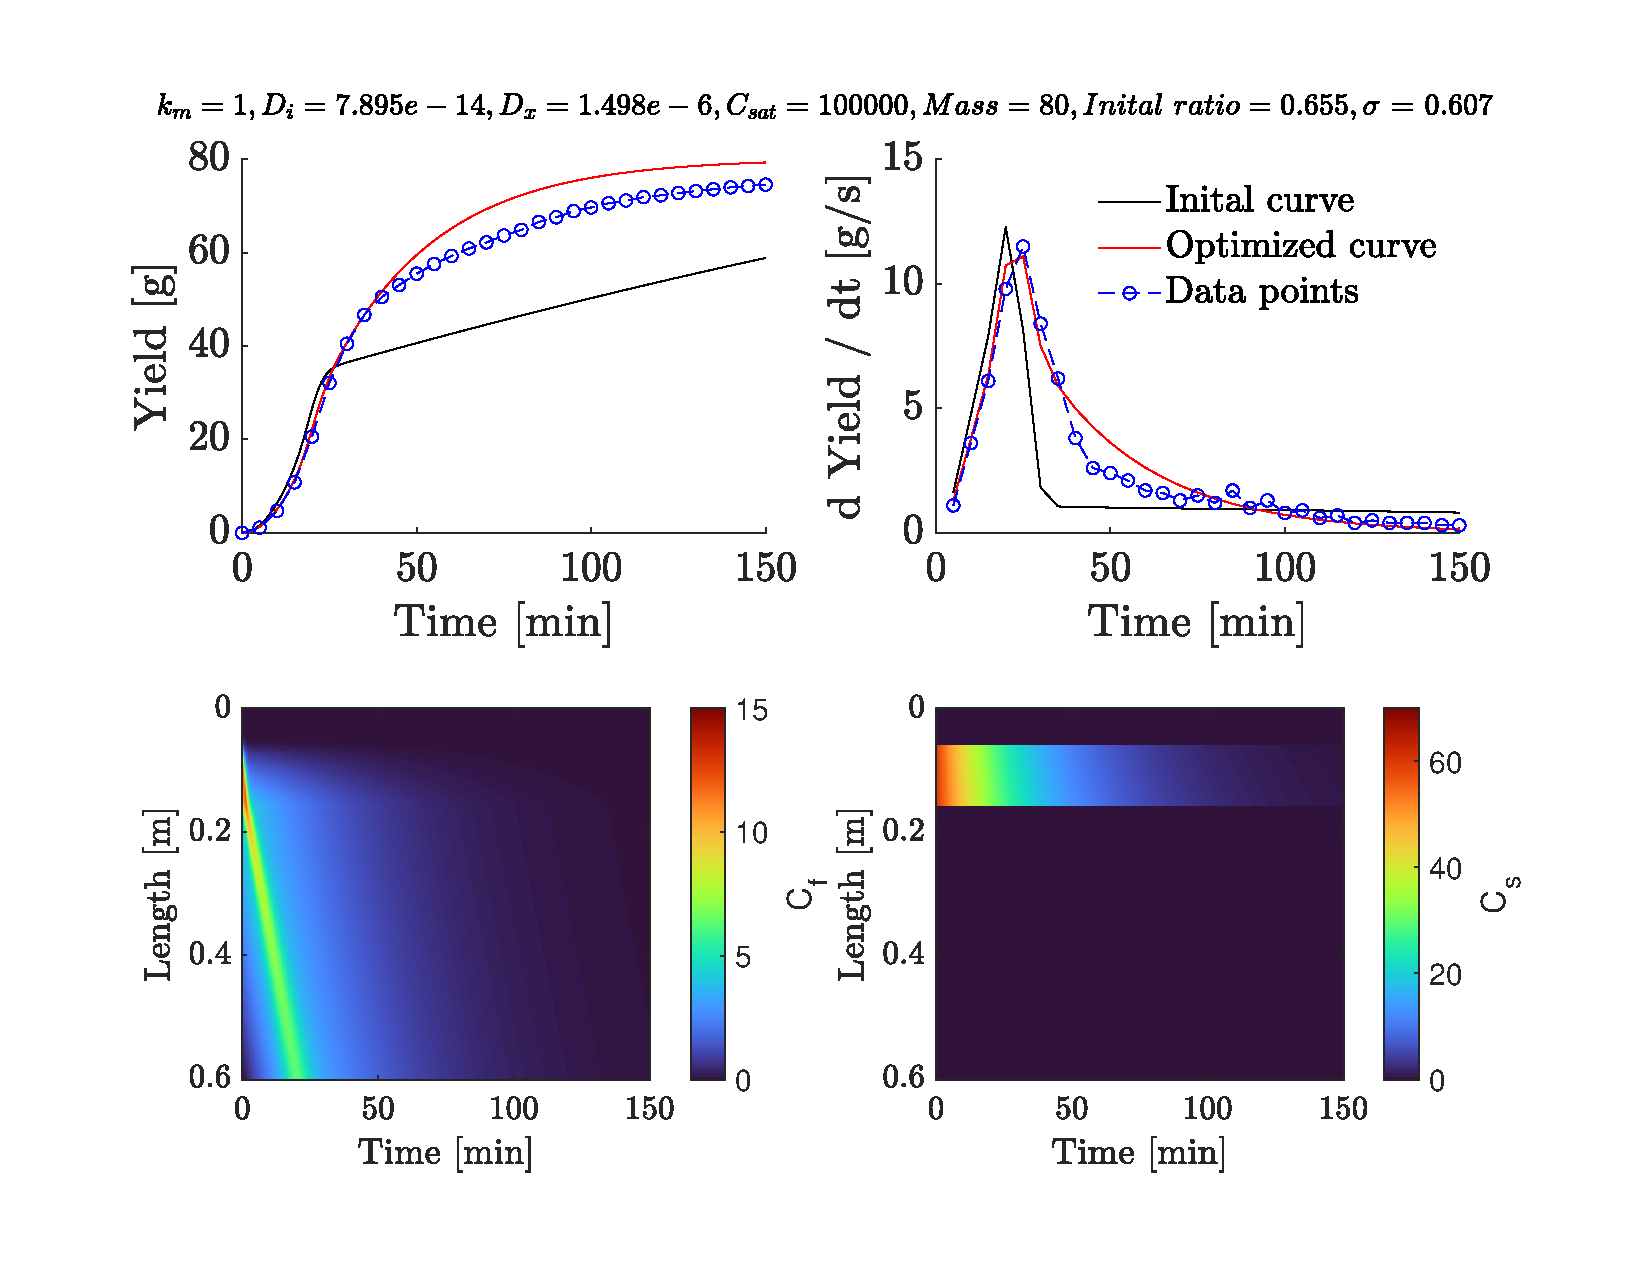
\includegraphics[trim = 2cm 1.4cm 1.9cm 11cm,clip,width=\textwidth]{/Results_estimation/Fitting_LUKE_T40_P300_org_2.pdf}
			\caption{Experiment at $40^\circ C$ and $300$ bar}
		\end{subfigure}
		\begin{subfigure}[b]{\columnwidth}
			\centering
			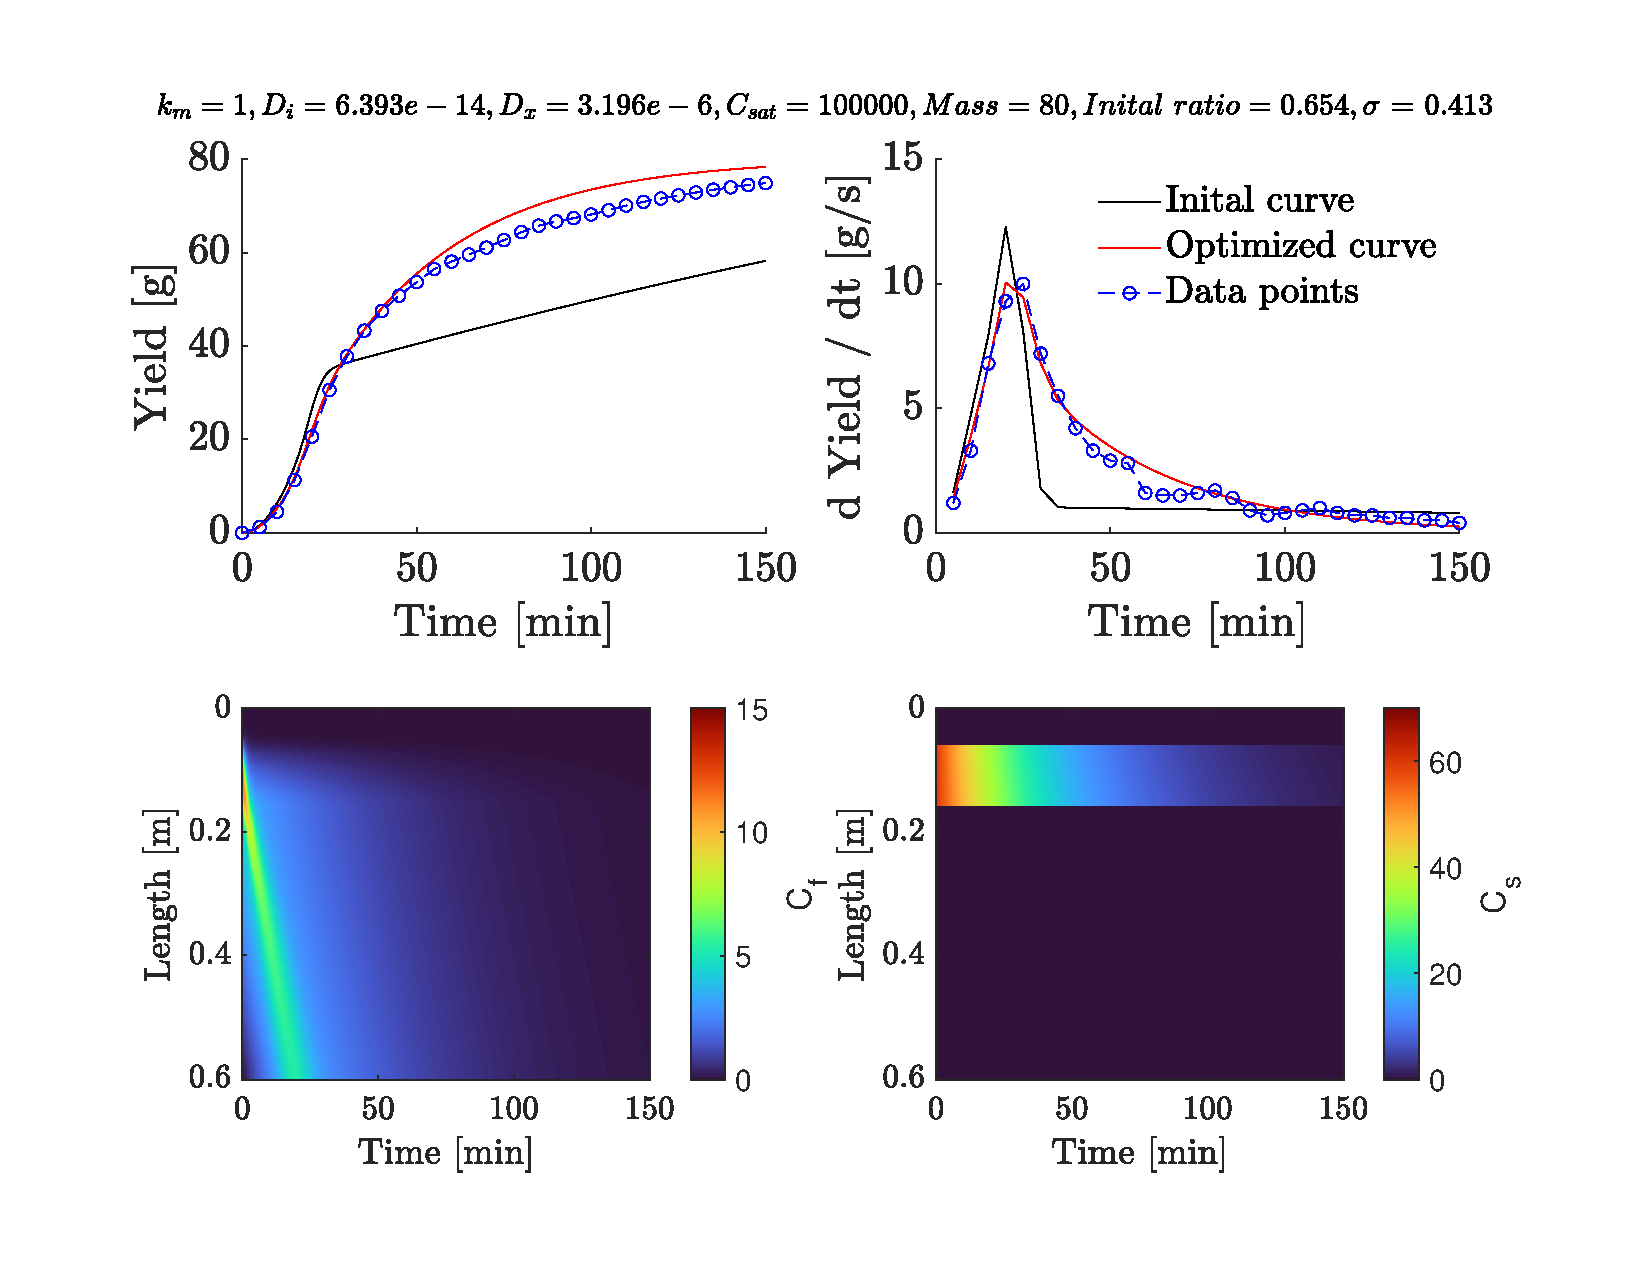
\includegraphics[trim = 2cm 1.4cm 1.9cm 11cm,clip,width=\textwidth]{/Results_estimation/Fitting_LUKE_T50_P300_org_2.pdf}
			\caption{Experiment at $50^\circ C$ and $300$ bar}
		\end{subfigure}
		\caption{Concentration profiles after solving the parameter estimation problem}
		\label{fig: estimation_results_profiles_2}
	\end{figure}
	
\end{document}